\section{Plant simulation results}

\subsection{Comparison with OpenRocket}

The plant simulation results are compared against the predictions from OpenRocket, focusing on several flight parameters. 
The comparisons were conducted under nominal conditions, with the simulation run for a flight trajectory without wind disturbances.
Even though the OR wind model is layed out in Niskanen \cite{niskanen2009}, the specific values for the stochastic turbulence are difficult to reproduce.

One simulation result from a simulated Borealis flight is shown in Fig. \ref{fig:result-or-comparison}. 
The horizontal axis represents time in seconds, and each subplot displays the time evolution of one of the flight parameters.
Note that the OR simulation deploys a parachute at apogee, which this plant model does not. 

\begin{figure}[ht]
    \centering
    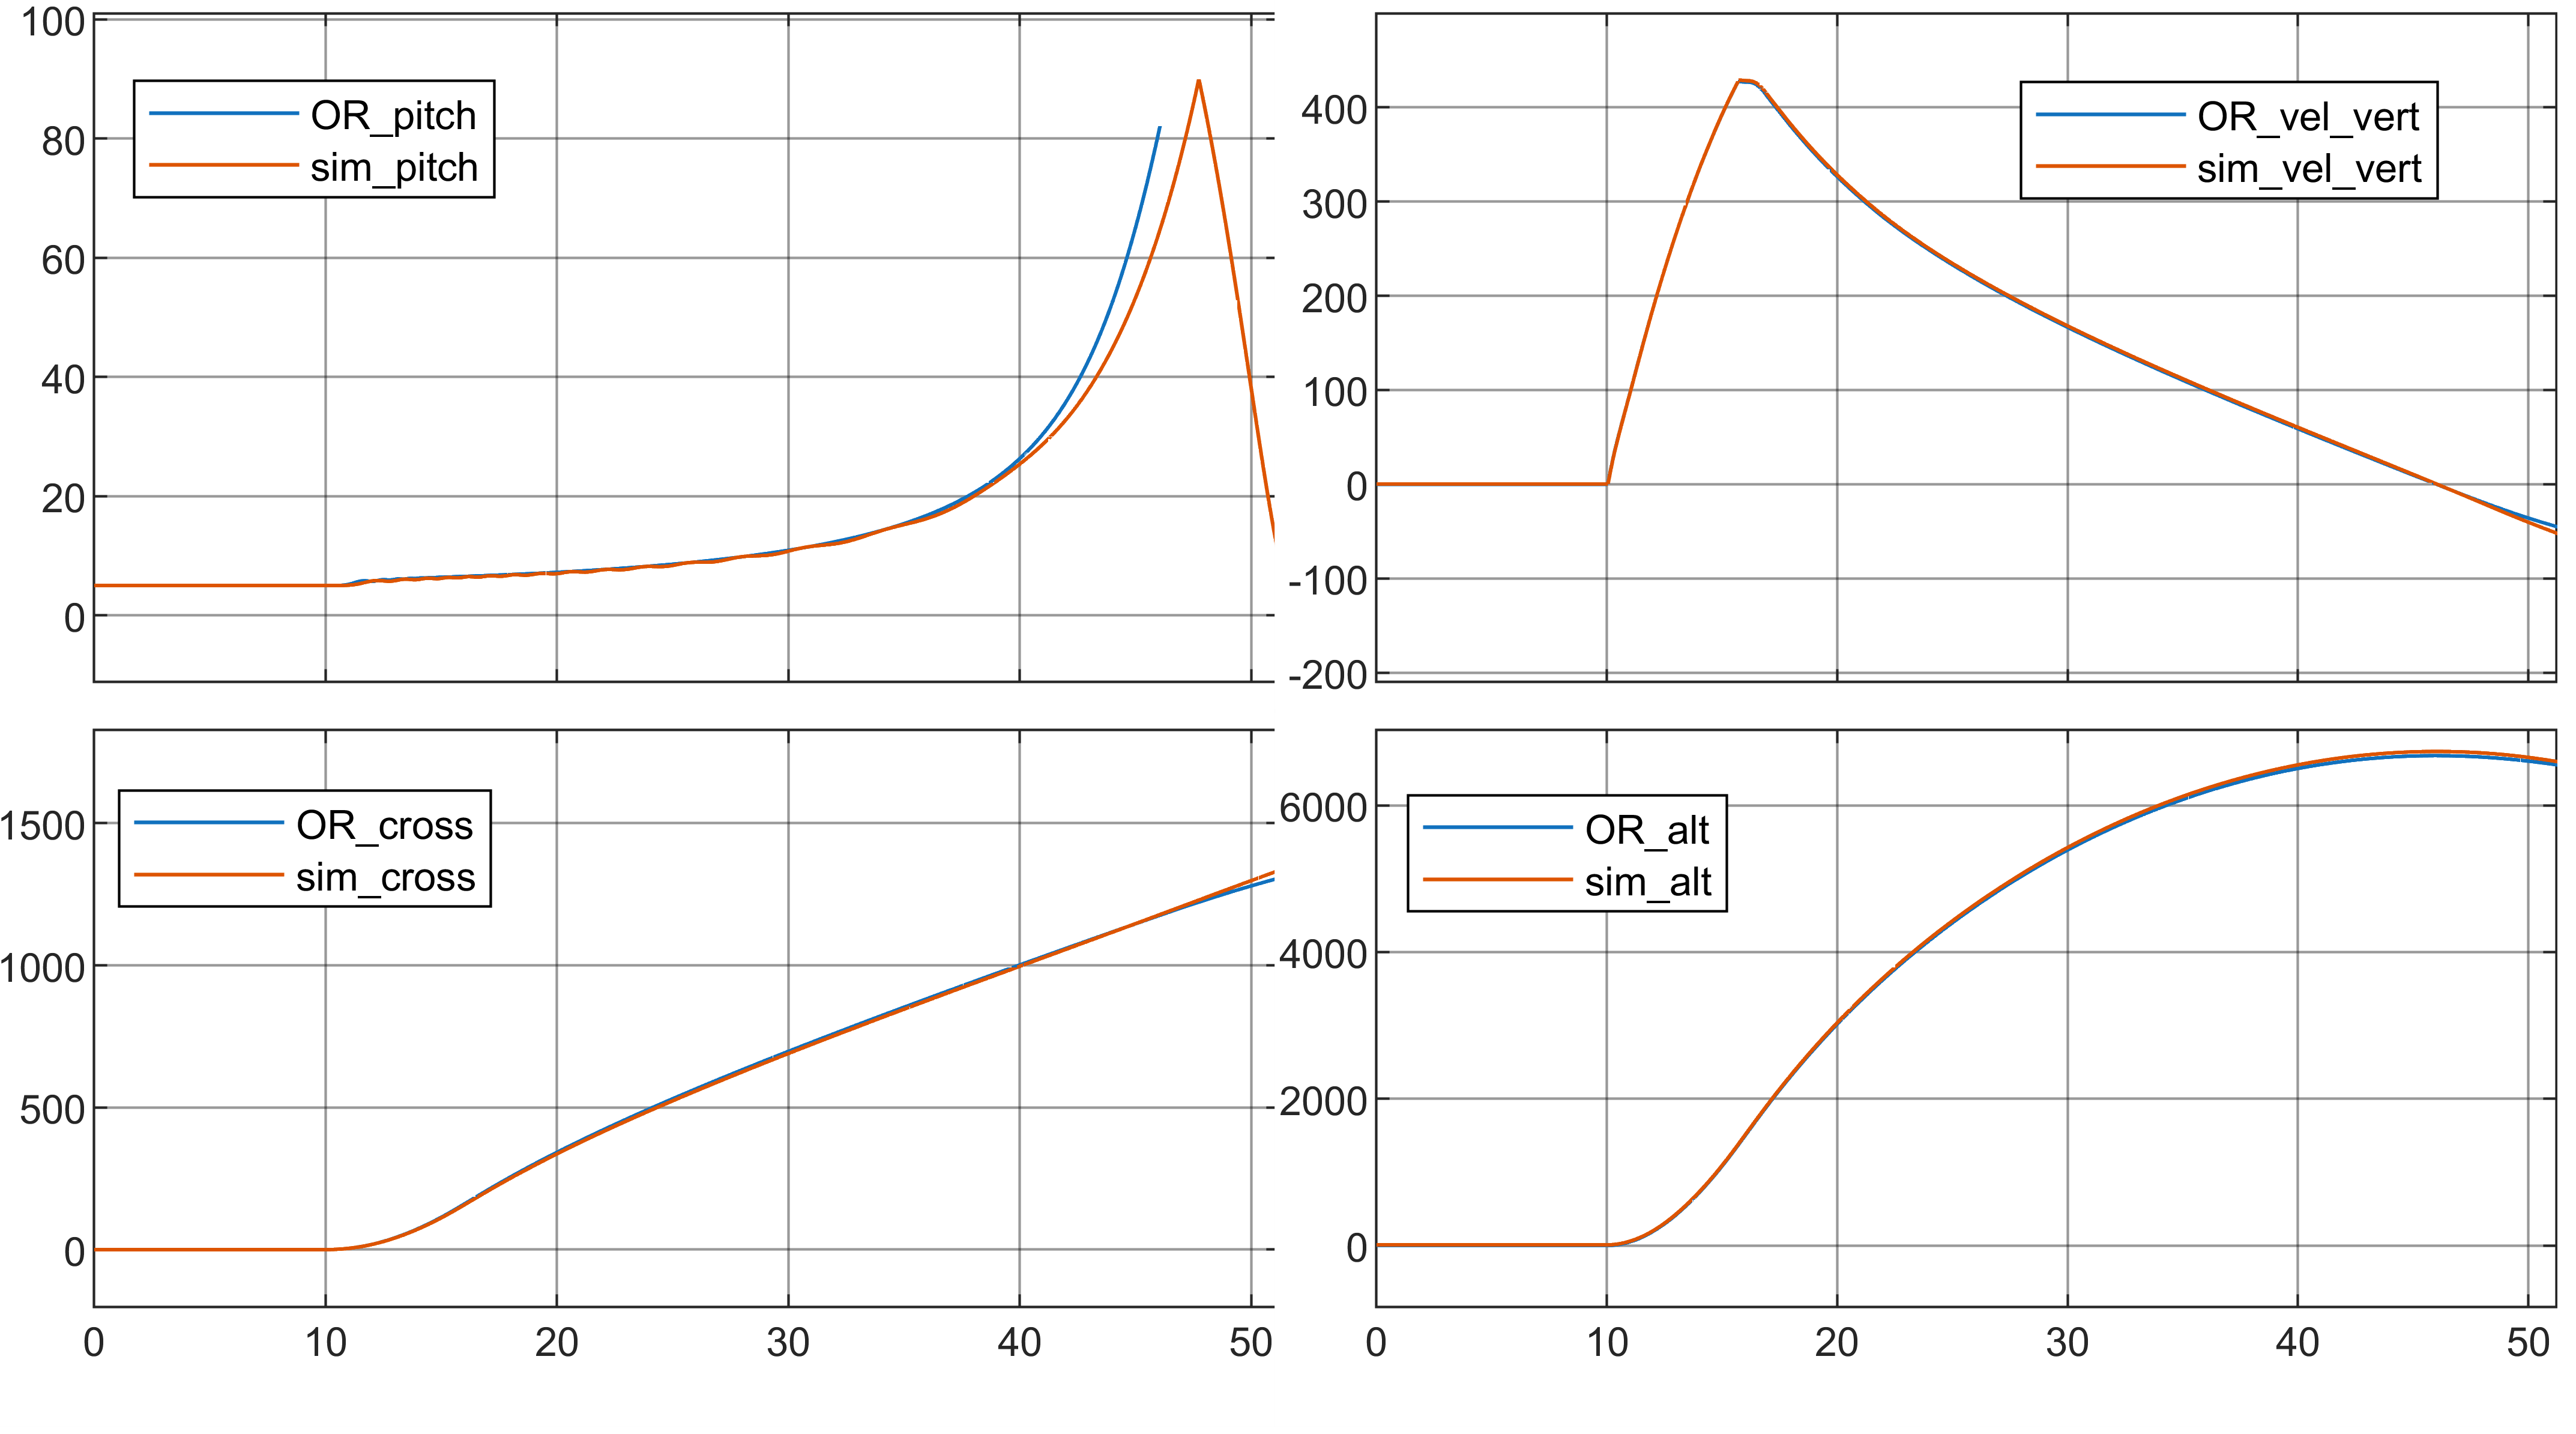
\includegraphics[width=0.95\linewidth]{images-plant/simulation_compare-OR.png}
    \caption[Simulation compared with OpenRocket]{Simulation results (red) compared with OpenRocket (blue), Borealis nominal flight. Common abscissa is time [s]. (Top Left) Pitch angle magnitude [deg], (Top Right) Vertical velocity [m/s], (Bottom Left) Cross range distance [m], (Bottom Right) Altitude [m].}
    \label{fig:result-or-comparison}
\end{figure}

The pitch angle trajectory from the simulation shows a similar trend to the OpenRocket results, indicating that the simulation captures the overall pitch dynamics of the rocket. 
However, the pitch angle in OR increases faster than this plant model, leading to a large deviation close to apogee.
Additionally, a pitch oscillation occurs shortly after liftoff, where OR shows a faster response than this model.
Both phenomena could be explained by significant differences in the pitch damping computation.
    
Both the simulation and OpenRocket predict a nearly identical profile for vertical velocity. 
This is due to the shared thrust curve between the models, and that the plant pre-processing creates an accurate $C_d$/Mach look-up table from the OR export.
As the pitch angle is very similar during powered ascent (10s until 15s), the thrust acts in the same proportion to the vertical acceleration.

The cross-range distance, which measures the lateral displacement of the rocket from its launch point, is also very similar.
As no wind disturbances were added, this is to be expected.
    
The altitude profiles from both the simulation and OpenRocket are almost identical during ascent, but diverge slightly near apogee.
This is due to a small accumulated difference in the vertical velocity.  

Overall, the simulation shows good agreement with OpenRocket across all measured parameters, validating the accuracy of the plant model under the conditions tested.